\begin{figure}[h]
    \centering
    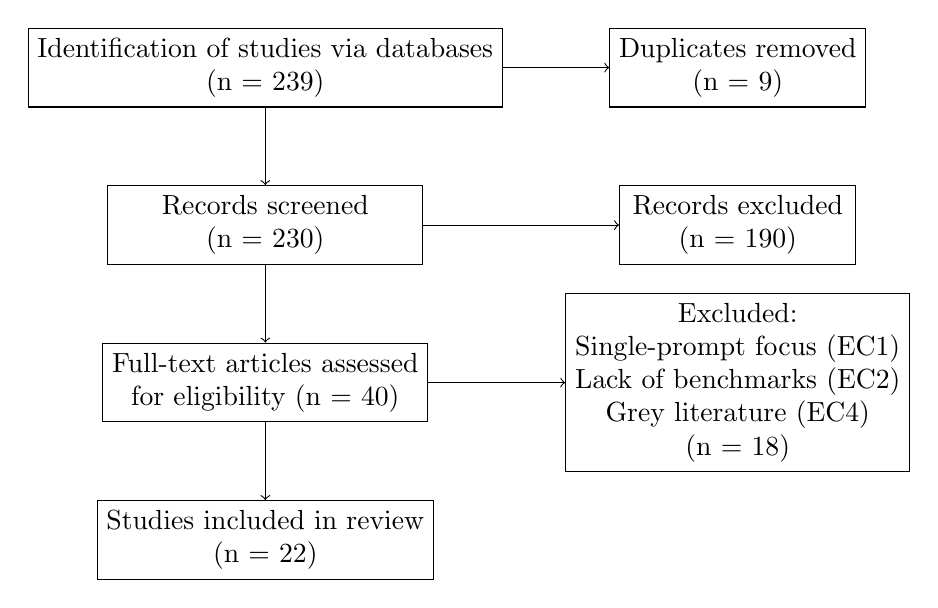
\begin{tikzpicture}[node distance=2cm]
        \node (identification) [draw, rectangle, minimum width=4cm, minimum height=1cm, align=center] {Identification of studies via databases\\(n = 239)};
        \node (screening) [draw, rectangle, below of=identification, minimum width=4cm, minimum height=1cm, align=center] {Records screened\\(n = 230)};
        \node (duplicates) [draw, rectangle, right of=identification, xshift=4cm, minimum width=3cm, minimum height=1cm, align=center] {Duplicates removed\\(n = 9)};
        \node (excluded_screen) [draw, rectangle, right of=screening, xshift=4cm, minimum width=3cm, minimum height=1cm, align=center] {Records excluded\\(n = 190)};
        \node (eligibility) [draw, rectangle, below of=screening, minimum width=4cm, minimum height=1cm, align=center] {Full-text articles assessed\\for eligibility (n = 40)};
        \node (excluded_full) [draw, rectangle, right of=eligibility, xshift=4cm, minimum width=3cm, minimum height=1cm, align=center] {Excluded:\\Single-prompt focus (EC1)\\Lack of benchmarks (EC2)\\Grey literature (EC4)\\(n = 18)};
        \node (included) [draw, rectangle, below of=eligibility, minimum width=4cm, minimum height=1cm, align=center] {Studies included in review\\(n = 22)};

        \draw[->] (identification) -- (screening);
        \draw[->] (identification) -- (duplicates);
        \draw[->] (screening) -- (eligibility);
        \draw[->] (screening) -- (excluded_screen);
        \draw[->] (eligibility) -- (included);
        \draw[->] (eligibility) -- (excluded_full);
    \end{tikzpicture}
    \caption{PRISMA 2020 Flow Diagram for the Systematic Literature Review.}
    \label{fig:prisma_flow}
\end{figure}
